\documentclass{article}

\usepackage{graphicx}
\usepackage{tikz}
\usepackage{tikzsymbols}
\usetikzlibrary{calc,patterns,shapes.geometric}
\pagestyle{empty}
\usepackage[margin=0pt]{geometry}
\geometry{papersize={14in,12in}}

\def\centerarc[#1](#2)(#3:#4:#5){\draw[#1] ($(#2)+({#5*cos(#3)},{#5*sin(#3)})$) arc (#3:#4:#5);}

\begin{document}
	\begin{figure}
		\centering
		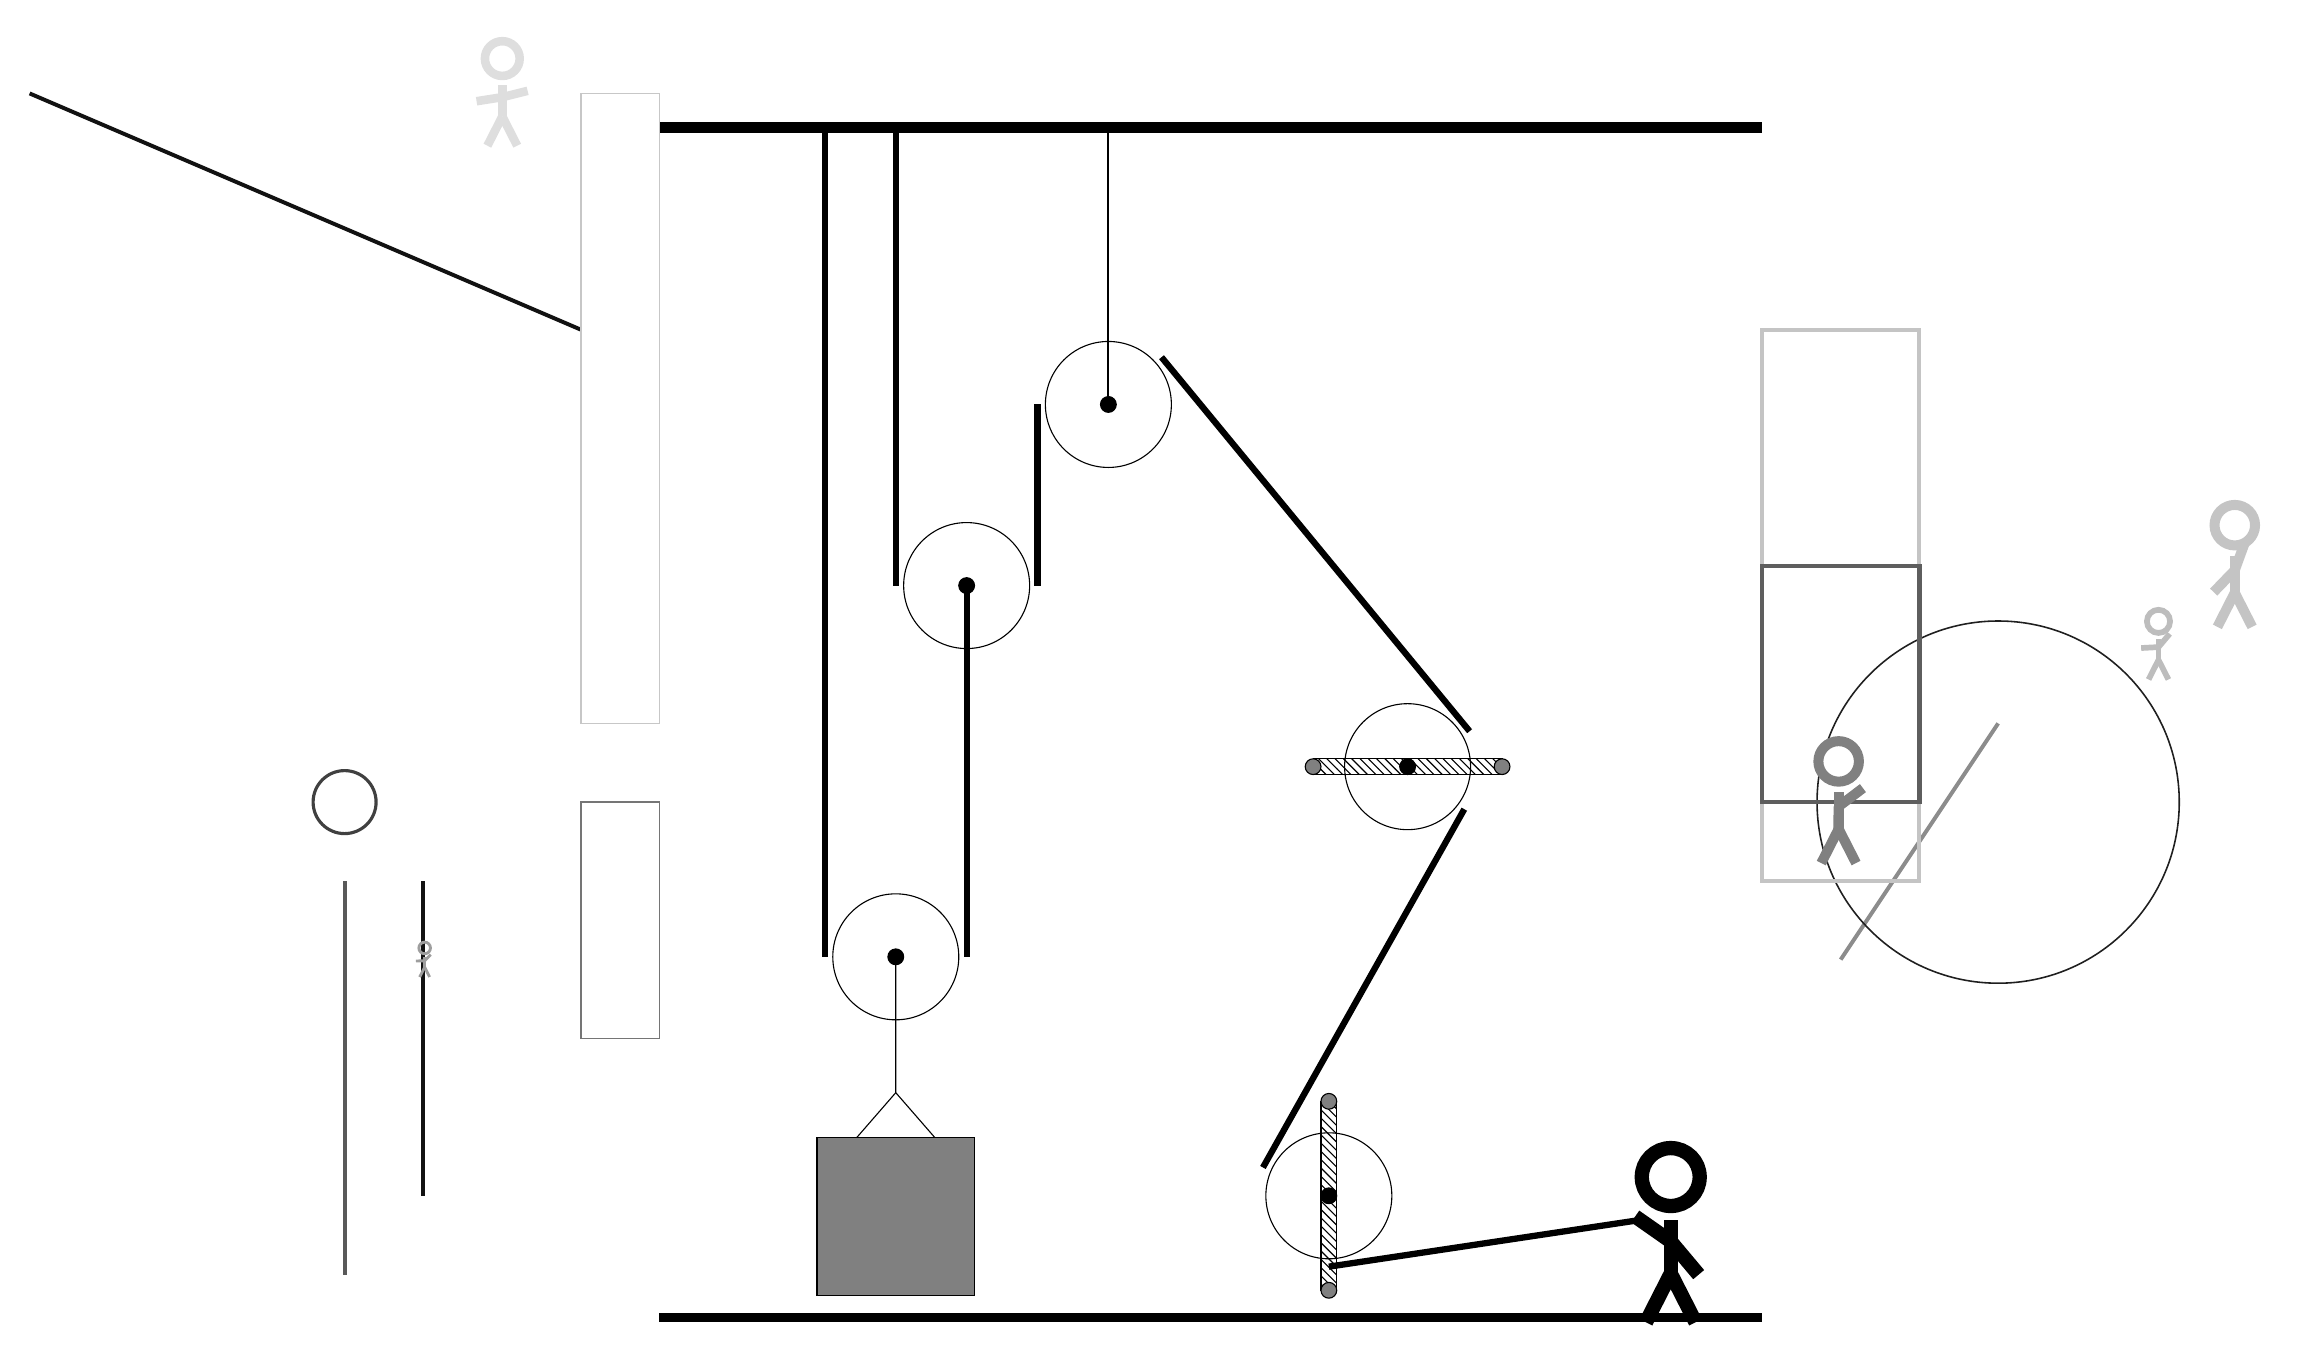
\begin{tikzpicture}
			%%%%% START %%%%%
			
			\draw[fill=black] (-2, 11.5) rectangle (12, 11.625);
			
			\draw (1, 1.035) circle (0.8);
			\draw[fill=black] (1, 1.035) circle (0.1);
			
			\draw (1.9, 5.75) circle (0.8);
			\draw[fill=black] (1.9, 5.75) circle (0.1);
			
			\draw (3.7, 8.05) circle (0.8);
			\draw[fill=black] (3.7, 8.05) circle (0.1);
			\draw[thick] (3.7, 8.05) -- (3.7, 11.5);
			
			\draw (6.5, -2) circle (0.8);
			\draw[fill=black] (6.5, -2) circle (0.1);
			\draw[pattern=north west lines, pattern color=black] (6.4, -0.8) rectangle (6.6, -3.2);
			\draw[fill=black!50] (6.5, -0.8) circle (0.1);
			\draw[fill=black!50] (6.5, -3.2) circle (0.1);
			
			\draw (7.5, 3.45) circle (0.8);
			\draw[fill=black] (7.5, 3.45) circle (0.1);
			\draw[pattern=north west lines, pattern color=black] (6.3, 3.55) rectangle (8.7, 3.35);
			\draw[fill=black!50] (6.3, 3.45) circle (0.1);
			\draw[fill=black!50] (8.7, 3.45) circle (0.1);
			
			\draw[line width=0.5mm, color=black!45](15, 4) -- (13, 1);
			
			\draw [line width=0.4mm, color=black!75](-6, 3) circle (0.4);
			\draw [line width=0.2mm, color=black!88](15, 3) circle (2.3);
			\draw[line width=0.2mm, color=black!54] (-3, 3) rectangle (-2, 0);
			\draw[line width=0.5mm, color=black!23] (12, 2) rectangle (14, 9);
			
			\draw[line width=0.6mm, color=black!63] (12, 3) rectangle (14, 6);
			\draw[line width=0.5mm, color=black!65](-6, -3) -- (-6, 2);
			\draw[line width=0.5mm, color=black!93](-5, -2) -- (-5, 2);
			\draw[line width=0.5mm, color=black!93](-3, 9) -- (-10, 12);
			\node[line width=0.4mm, color=black!23] at (18, 6) {\Strichmaxerl[7][46][70]};
			\node[line width=0.3mm, color=black!38] at (-5, 1) {\Strichmaxerl[2][1][46]};
			\draw[line width=0.2mm, color=black!22] (-3, 12) rectangle (-2, 4);
			\node[line width=0.6mm, color=black!50] at (13, 3) {\Strichmaxerl[7][89][37]};
			
			\node[line width=0.4mm, color=black!26] at (17, 5) {\Strichmaxerl[4][3][50]};
			\node[line width=0.3mm, color=black!13] at (-4, 12) {\Strichmaxerl[6][9][14]};
			
			\draw (1, 1.035) -- (1, -0.69) -- (0.5, -1.265) -- (1.5, -1.265) -- (1, -0.69);
			\draw[fill=black!50] (0, -1.265) rectangle (2, -3.265);
			
			\draw[line width=0.8mm] (0.1, 11.5) -- (0.1, 1.035);
			\centerarc[line width=0.8mm](1, 1.035)(180:360:0.9);
			\draw[line width=0.8mm](1.9, 1.035) -- (1.9, 5.75);
			\draw[line width=0.8mm] (1.0, 11.5) -- (1.0, 5.75);
			\centerarc[line width=0.8mm](1.9, 5.75)(180:360:0.9);
			\draw[line width=0.8mm](2.8, 5.75) -- (2.8, 8.05);
			\centerarc[line width=0.8mm](3.7, 8.05)(35:180:0.9);
			\draw[line width=0.8mm] (4.375, 8.65) -- (8.2875, 3.9);
			\centerarc[line width=0.8mm](7.5, 3.45)(215:135:-0.9);
			\draw[line width=0.8mm](8.22, 2.91) -- (5.663, -1.64);
			\centerarc[line width=0.8mm](6.5, -2)(-30:100:-0.9);
			\draw[line width=0.8mm](6.5, -2.9) -- (10.5, -2.3);
			
			\node at (10.8, -2.5) {\Strichmaxerl[10][-35][-50]};
			
			\draw[fill=black] (-2, -3.5) rectangle (12, -3.6);
			
			%%%%% END %%%%%
		\end{tikzpicture}
	\end{figure}	
\end{document}